\begin{figure}[h!]
    \centering
    \caption{Effects of \emph{Plan Cuadrante} Using a Balanced Panel of Municipalities}
    \label{fig:figureA6_bp}
    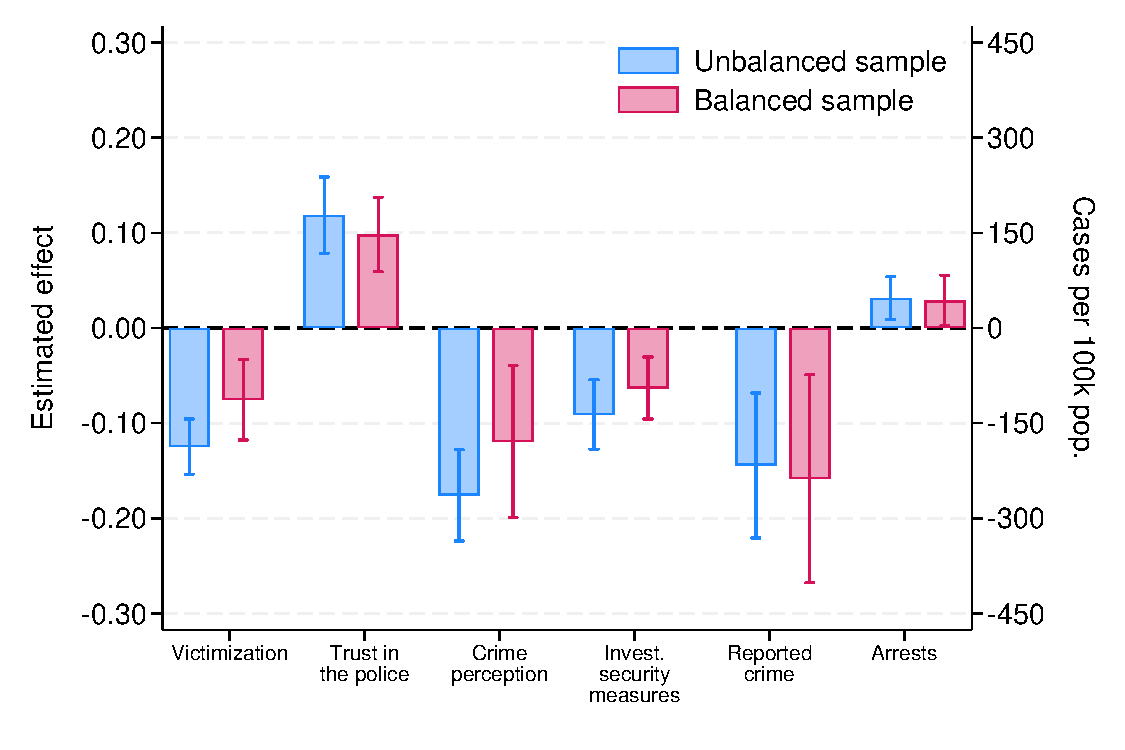
\includegraphics[width=0.8\textwidth]{../manuscript/Graphs/results_crime_balanced_combined.pdf}
    \\[10pt]
    \begin{minipage}{0.99\textwidth}
    \footnotesize Notes: The figure reports the effects of \emph{Plan Cuadrante} on different measures of police effectiveness using the main analytical sample (unbalanced, blue bars) and a balanced panel of municipalities observed over the full event-study window from $t-2$ to $t+3$ (red bars). For the ENUSC sample the balanced panel consists of the 31 municipalities that implemented \emph{Plan Cuadrante} between 2006 and 2009; for the administrative municipality-level sample it consists of 94 municipalities for reported crime and 78 municipalities for arrests. The bars represent the average post-treatment effect estimated with the difference-in-differences estimator developed in \citet{Callaway}, and the whiskers the 95\% confidence intervals; standard errors are clustered at the municipality level. Victimization is the probability of household victimization in the last 12 months; reported crime is the number of crimes reported to the police in the municipality per 100,000 inhabitants; arrests is the number of arrests per 100,000 inhabitants; trust in the police is the probability of reporting high trust in the police; crime perception is the probability of perceiving an increase in crime; and investment in security measures is the probability of adopting security measures in the last twelve months. Reported crime and arrests (administrative data) are read on the right axis; all other outcomes, from the ENUSC survey, are read on the left axis.
    \end{minipage}
\end{figure}
